\chapter{Implementing the Metropolis Acceptance Criteria}

All Monte Carlo moves are implemented in Cassandra to preserve detailed balance between each pair of microstates $m$ and $n$
\begin{equation}
\label{eq:detailedBalance}
\Pi_{mn}\ \alpha_{mn}\ p_m = \Pi_{nm}\ \alpha_{nm}\ p_n
\end{equation}
where $\Pi_{mn}$ is the probability of accepting the move from microstate $m$ to microstate $n$, $\alpha_{mn}$ is the probability of attempting the move that will form $n$ from $m$, and $p_m$ is the probability of $m$ in the ensemble of interest.

In Cassandra, detailed balance is enforced via the Metropolis criterion
\begin{equation}
\label{eq:metropolis}
\Pi_{mn} = \min\left(1, \frac{\alpha_{nm}}{\alpha_{mn}} \frac{p_n}{p_m} \right)
\end{equation}
The ratio in Eq.\ (\ref{eq:metropolis}) will often involve an exponential, e.g. $e^{-\beta \Delta U}$. To preserve precision in the energy calculation, the acceptance probability is computed
\begin{equation}
\label{eq:metropolis_2}
\Pi_{mn} = \exp\left\{-\max\left[0, \ln\left(\frac{\alpha_{mn}}{\alpha_{nm}} \frac{p_m}{p_n}\right)\right]\right\}
\end{equation}
The logarithm, defined in code as ln\_pacc, is tested in the function accept\_or\_reject() which is defined in file accept\_or\_reject.f90. If ln\_pacc is greater than 0 and less than a maximum numerical value, $\Pi_{mn}$ is computed and compared to a random number.

\begin{minipage}{\linewidth}
\begin{lstlisting}[firstnumber=47, caption=accept\_or\_reject.f90]
  accept = .FALSE.

  IF (ln_pacc <= 0.0_DP) THEN

     accept = .TRUE.

  ELSE IF ( ln_pacc < max_kBT) THEN

     pacc = DEXP(-ln_pacc)

     IF ( rranf() <= pacc ) THEN
         
        accept = .TRUE.

     END IF

  END IF
\end{lstlisting}
\end{minipage}

\section{Canonical Monte Carlo}
\label{sec:NVT}
In the canonical ensemble, the number of molecules $N$, the volume $V$ and temperature $T$ are all constant. The position, orientation and conformation of a semi-flexible molecule with fixed bond-lengths containing $M$ atoms is given by a 2$M$+1-dimensional vector $\mathbf{q}$. The positions, orientations and conformations of all $N$ molecules are denoted $\mathbf{q}^N$.

The probability of observing microstate $m$ with configuration $\mathbf{q}_m^N$ is
\begin{equation}
\label{eq:pNVT}
p_m = \frac{e^{-\beta U\left(\mathbf{q}_m^N\right)}}{Z(N,V,T)}\ d\mathbf{q}^N
\end{equation}
where $\beta$ is the inverse temperature $1/k_BT$, $U$ is the potential energy, the differential volume $d\mathbf{q}^N$ is included to make $p_m$ dimensionless and $Z$ is the configurational partition function
\begin{equation}
\label{eq:configPartitionFn_NVT}
Z(N,V,T) = \int e^{-\beta U(\mathbf{q}^N)} d\mathbf{q}^N.
\end{equation}
The integral is over all $N(2M+1)$ degrees of freedom. The ratio of microstate probabilities follows from Eq.\ (\ref{eq:pNVT})
\begin{align}
\label{eq:pNVT_ratio}
\frac{p_m}{p_n} &= \frac{e^{-\beta U\left(\mathbf{q}_m^N\right)} d\mathbf{q}^N/Z(N,V,T)}{e^{-\beta U\left(\mathbf{q}_n^N\right)} d\mathbf{q}^N/Z(N,V,T)} \nonumber \\
&= e^{\beta (U_n - U_m)} = e^{\beta \Delta U}
\end{align}
The configurational partition function $Z$ and differential volume $d\mathbf{q}^N$ both cancel, leaving only the ratio of Boltzmann factors.

New configurations are generated by attempting moves that translate, rotate and regrow a randomly selected molecule.

\subsection{Translating a Molecule}
\label{sec:translate}
A molecule is translated by moving its center of mass in each Cartesian direction by a random amount chosen from the uniform distribution on the interval [-$\delta r_{max},\delta r_{max}$]. The maximum displacement $\delta r_{max}$ must be given in the input file. The translation move is symmetric in forward and reverse directions. That is, either microstate $n$ can be formed from microstate $m$ and vice versa by moving one molecule within $\delta r_{max}$ in each Cartesian direction, or microstate $n$ cannot be formed at all. As a result, $\alpha_{mn} = \alpha_{nm}$.

The acceptance probability for a translation move follows from Eq.\ (\ref{eq:pNVT_ratio})
\begin{equation}
\label{eq:pAcc_translate}
\ln \left( \frac{\alpha_{mn}}{\alpha_{nm}} \frac{p_m}{p_n} \right) = \ln \left( \frac{p_m}{p_n} \right) = \beta \Delta U
\end{equation}

In Cassandra, the translation move is implemented in the subroutine Translate defined in translate.f90. The relevant lines from version 1.1 are quoted below. The variable names in the translate.f90 code are identified with the symbols from Eq.\ (\ref{eq:pAcc_translate}) in Table \ref{table:translate}.

\begin{lstlisting}[firstnumber=274, caption=translate.f90, label=code:translate]
ln_pacc = beta(this_box) * delta_e
accept = accept_or_reject(ln_pacc)
\end{lstlisting}

\begin{table}
\caption{Variable symbols and code names for translating and rotating a molecule}
\label{table:translate}
\centering
\begin{tabular}{|c|c|} \hline
 {\bf Symbol} & {\bf Code name} \\ \hline
 $\beta$ & beta(this\_box) \\
 $\Delta U$ & delta\_e \\
 \hline
\multicolumn{2}{c}{}
\end{tabular}
\end{table}

\subsection{Rotating a Molecule}
\label{sec:rotate}
A linear molecule is rotated differently than a nonlinear molecule. A molecule is identified as linear if it is composed of 2 atoms or if all the angles are rigid with a bond angle of 180$\degree$. If the molecule is linear: 

\begin{enumerate}
	\item Pick three random angles: $\phi$ on [$-\pi,\pi$], $\cos(\theta)$ on [-1,1], and $\psi$ on [$-\pi,\pi$].
	\item With the origin at the molecule's center of mass, rotate by $\phi$ around $z$, rotate by $\theta$ around $x'$, and rotate by $\psi$ around $z'$, as shown in Fig. \ref{fig:EulerAngles}.
\end{enumerate}

Even though three angles are randomly chosen, the probability of the resulting orientation is $d\cos(\theta)d\phi/4\pi$.

\begin{figure}[h]
	\centering
	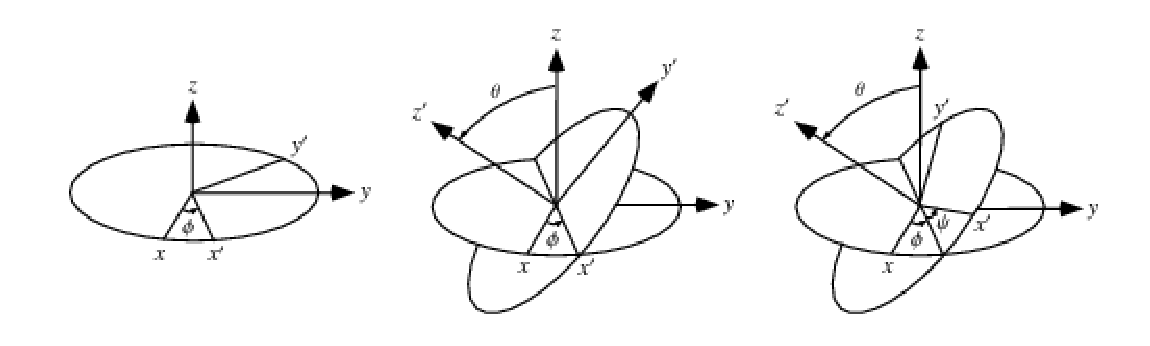
\includegraphics[width=0.9\textwidth]{EulerAngles}
	\caption{Procedure for rotating linear molecules. \newline Image from mathworld.wolfram.com/EulerAngles.html.}
	\label{fig:EulerAngles}
\end{figure}

If the molecule is nonlinear:

\begin{enumerate}
	\item Randomly select an axis: $x$, $y$, or $z$.
	\item Choose a random angular displacement $\delta \theta$ from $[-\delta \theta_{max}, \delta \theta_{max}]$. $\delta \theta_{max}$ must be given in the input file.
	\item Rotate the molecule around a vector parallel to the selected axis and through its center of mass by $\delta \theta$.
\end{enumerate}

In either case, the rotation move is symmetric, $\alpha_{mn} = \alpha_{nm}$, and the acceptance criteria is given by Eq.\ (\ref{eq:pAcc_translate}). The rotation move is implemented in subroutine Rotate defined in rotate.f90.

\begin{lstlisting}[firstnumber=261, caption=rotate.f90, label=code:rotate]
ln_pacc = beta(this_box) * delta_e
accept = accept_or_reject(ln_pacc)
\end{lstlisting}

\subsection{Regrowing a Molecule}
\label{sec:regrow}
Internal degrees of freedom in flexible molecules are sampled by deleting one or more fragments from the molecule and replacing the deleted fragments with conformations from a reservoir of fragment conformations. If the molecule consists of only a single fragment (e.g, water, all atom methane, united atom propane, all atom cyclohexane), the entire molecule is deleted and replaced as follows:

\begin{enumerate}
	\item Randomly select a molecule $i$ with uniform probability $1/N$, record its center-of-mass position and delete it.
	\item Select a molecular conformation with Boltzmann probability $e^{-\beta U(\mathbf{q}_{int,n}^{(i)})}/Z_{int}$, where $\mathbf{q}_{int,n}^{(i)}$ are the internal bond or improper angles of molecule $i$ in microstate $n$ and $Z_{int}$ is the configurational partition function over internal degrees of freedom (see Eq. (\ref{eq:configPartitionFn_1VT})).
	\item Pick three random angles: $\phi$ on [$-\pi,\pi$], $\cos(\theta)$ on [-1,1], and $\psi$ on [$-\pi,\pi$]. Rotate the molecule as shown in Fig. \ref{fig:EulerAngles}. The probability of the resulting orientation is $d\mathbf{q}_{rot}/Z_{rot}$, which for a nonlinear molecule is $d\cos(\theta) d\phi d\psi / 8 \pi^2$.
	\item Place the molecule with the selected conformation and orientation at the same center-of-mass position as the deleted molecule.
\end{enumerate}

Regrowing a monoatomic particle has no effect. Regrowing a linear molecule is the same as rotating it. The overall probability $\alpha_{mn}$ of regrowing a molecule with the selected orientation and conformation is 

\begin{equation}
\label{eq:alpha_regrow}
\alpha_{mn} = \frac{1}{N} \frac{d\mathbf{q}_{rot}}{Z_{rot}} \frac{e^{-\beta U(\mathbf{q}_n^{(i)})}d\mathbf{q}_{int}}{Z_{int}}
\end{equation}

where $\mathbf{q}_n^{(i)}$ denotes the position, orientation and conformation of molecule $i$ in microstate $n$ and $U(\mathbf{q}_n^{(i)})$ is the potential energy of the isolated molecule $i$, i.e. the intramolecular potential energy. The reverse probability $\alpha_{nm}$ is identical except for the intramolecular potential energy $U(\mathbf{q}_m^{(i)})$ of molecule $i$ in microstate $m$. Using Eqs. (\ref{eq:pNVT_ratio}) and (\ref{eq:alpha_regrow}), the acceptance criteria for the regrowth of a single fragment molecule is

\begin{align}
\label{eq:pAcc_regrow}
\ln\left( \frac{\alpha_{mn}}{\alpha_{nm}} \frac{p_m}{p_n} \right) &= \beta \left[\left(U(\mathbf{q}^N_n) - U(\mathbf{q}^N_m)\right) - \left( U(\mathbf{q}_n^{(i)}) - U(\mathbf{q}_m^{(i)})\right)\right] \\ \nonumber
&= \beta \Delta U - \beta \Delta U_{int}^{(i)} = \beta \Delta U_{inter}^{(i)}
\end{align}

Only the change in the intermolecular potential energy between molecule $i$ and the other $N-1$ molecules contributes to the acceptance criteria. The code that implements Eq. (\ref{eq:pAcc_regrow}) is shown in Code \ref{code:cbmcRegrow} in Section \ref{sec:cbmcRegrow}.

If the molecule consists of more than one fragment (e.g., all atom ethane, all atom toluene, united atom butane), a bond is cut and the severed fragments are regrown using Configurational Bias Monte Carlo (CBMC). See Section \ref{sec:cbmcRegrow} for more details.

\subsection{Canonical Partition Function}
In Sections \ref{sec:translate}-\ref{sec:rotate}, the microstate probability is normalized by the configuration partition function $Z$ because the only relevant degrees of freedom are configurational. In other ensembles, the full partition function $Q$ appears, integrated over both configuration space $\mathbf{q}^N$ and momenta space $\mathbf{p}_q^N$

\begin{equation}
\label{eq:partitionFn_NVT}
Q(N,V,T) = \frac{1}{h^{N(2M+1)} N!} \int e^{-\beta H(\mathbf{p}_q^N, \mathbf{q}^N)}\ d\mathbf{p}_q^N d\mathbf{q}^N
\end{equation}

where the 2$M$+1 momenta $\mathbf{p}_q$ are conjugate to the generalized coordinates $\mathbf{q}$. The momenta and configuration integrals are separable, and the single molecule momenta integrals are all identical.

\begin{align}
Q(N,V,T) &= \frac{1}{N!} \left[\int e^{-\beta U(\mathbf{q}^N)} d\mathbf{q}^N \right] \left[\frac{1}{h^{2M+1}} \int e^{-\beta K(\mathbf{p}_q)}\ d\mathbf{p}_q \right]^N \nonumber \\
&= \frac{1}{N!} Z(N,V,T) \left[\frac{Q(1,V,T)}{Z(1,V,T)}\right]^N
\end{align}

where $Q(1,V,T)$ is the partition function of a single molecule in a box. The center of mass integrals for a single molecule are separable from the integrals over rotational and internal degrees of freedom:

\begin{equation}
\label{eq:partitionFn_1VT}
Q(1,V,T) = Q_{com}Q_{rot+int} = V \Lambda^{-3} Q_{rot+int}
\end{equation}

where $\Lambda$ is the de Broglie wavelength of the molecule and the rotational and internal momenta integratals in $Q_{rot+int}$ are not separable since the moments of inertia will depend on the conformation adopted by the molecule. The configurational partition function is further separable into center of mass (translational), orientational and internal degrees of freedom:

\begin{equation}
\label{eq:configPartitionFn_1VT}
Z(1,V,T) = VZ_{rot}Z_{int}
\end{equation}

where the volume $V$ is the translational partition function and $Z_{rot}$ equals 4$\pi$ for a linear molecule and 8$\pi^2$ for a nonlinear molecule.

\section{Isothermal-Isobaric Monte Carlo}
\label{sec:NPT}
In the isothermal-isobaric ensemble, the number of particles $N$, the pressure $P$ and temperature $T$ are all constant while the volume $V$ and energy $E$ fluctuate. The partition function is

\begin{equation}
\label{eq:partitionFn_NPT}
\Delta(N,P,T) = \int e^{-\beta P V} Q(N,V,T) dV
\end{equation}

Note that $Q$ is dimensionless and $\Delta$ has dimensions of volume. The probability of the system having volume $V$ is 

\begin{equation}
\label{eq:pV}
p(V) = \frac{Q(N,V,T)e^{-\beta P V}}{\Delta(N,P,T)}dV
\end{equation}

The probability of observing microstate $m$ with configuration $\mathbf{q}_m^N$ and volume $V_m$ is

\begin{align}
\label{eq:pNPT}
p_m &= \frac{e^{-\beta U(\mathbf{q}_m^N)}d\mathbf{q}_m^N}{Z(N,V_m,T)}\ \frac{Q(N,V_m,T) e^{-\beta P V_m} dV}{\Delta(N,P,T)} \nonumber \\
&= \frac{e^{-\beta U_m - \beta P V_m}}{\Delta(N,P,T)}\ \left(\frac{Q(1,V_m,T)}{Z(1,V_m,T)}\ d\mathbf{q}_m\right)^N dV
\end{align}

where the differential volume element $d\mathbf{q}_m^N$ has subscript $m$ becuase it depends on the volume $V_m$. The ratio of microstate probabilities is

\begin{equation}
\label{eq:pNPT_ratio}
\frac{p_m}{p_n} = e^{\beta (U_n - U_m) + \beta P (V_n - V_m)} \left(\frac{d\mathbf{q}_m}{d\mathbf{q}_n}\right)^N = e^{\beta \Delta U + \beta P \Delta V} \left(\frac{d\mathbf{q}_m}{d\mathbf{q}_n}\right)^N
\end{equation}

\subsection{Scaling the Volume}
In Cassandra, new volumes are sampled as follows:

\begin{enumerate}
	\item Pick a random volume $\Delta V$ with uniform probability from the interval [$-\delta V_{max}$,\ $\delta V_{max}$]. The trial volume is $V + \Delta V$.
	\item Scale the box lengths uniformly.
	\item Scale the center of mass of each molecule uniformly.
\end{enumerate}

The probability of selecting $\Delta V$ is the same as selecting $-\Delta V$ which makes scaling the volume symmetric, $\alpha_{mn}=\alpha_{nm}$. Scaling the configurations changes the differential element $d\mathbf{q}_m^N$ surrounding configuration $\mathbf{q}_m^N$. Only the molecular centers of mass change, so we can separate $d\mathbf{q}$ into 3 center of mass coordinates $d\mathbf{r}_{com}$ and 2$M$-2 orientational and internal coordinates $d\mathbf{q}_{rot+int}$. The scaled center of mass positions are held constant, making $d\mathbf{r}_{com} = V d\mathbf{s}_{com}$. The acceptance probability for a volume scaling move is

\begin{equation}
\label{eq:pAcc_volume}
\ln \left( \frac{\alpha_{mn}}{\alpha_{nm}} \frac{p_m}{p_n} \right) = \ln \left( \frac{p_m}{p_n} \right) = \beta \Delta U + \beta P \Delta V + N \ln\left(\frac{V_m}{V_n}\right)
\end{equation}

The volume scaling move is implemented in subroutine Volume\_Change defined in volume\_change.f90. 

\begin{lstlisting}[firstnumber=475, caption=volume\_change.f90, label=code:volume]
ln_pacc = beta(this_box) * delta_e &
        + beta(this_box) * pressure(this_box) * delta_volume &
        - total_molecules * DLOG(box_list(this_box)%volume/box_list_old%volume)
accept = accept_or_reject(ln_pacc)
\end{lstlisting}

\begin{table}
\caption{Variable symbols and code names for volume scaling move.}
\label{table:volume}
\centering
\begin{tabular}{|c|c|} \hline
 {\bf Symbol} & {\bf Code name} \\ \hline
 $\beta$ & beta(this\_box) \\
 $\Delta U$ & delta\_e \\
 $P$ & pressure(this\_box) \\
 $\Delta V$ & delta\_volume \\
 $N$ & total\_molecules \\
 $V_n$ & box\_list(this\_box)\%volume \\
 $V_m$ & box\_list\_old\%volume \\
 \hline
\multicolumn{2}{c}{}
\end{tabular}
\end{table}


\section{Grand Canonical Monte Carlo}
\label{sec:MuVT}
In the grand canonical ensemble, the chemical potential $\mu$, the volume $V$ and temperature $T$ are held constant while the number of molecules $N$ and energy $E$ fluctuate. The partition function is 

\begin{equation}
\label{eq:partitionFn_MuVT}
\Xi(\mu,V,T) = \sum\limits_{N=0}^{\infty} Q(N,V,T)\ e^{\beta \mu N}
\end{equation}

The probability of the system having $N$ molecules is 

\begin{equation}
\label{eq:pN}
p(N) = \frac{Q(N,V,T)e^{\beta \mu N}}{\Xi(\mu,V,T)}
\end{equation}

The probability of observing microstate $m$ with $N_m$ molecules and configuration $\mathbf{q}_m^{N_m}$ is

\begin{align}
\label{eq:pMuVT}
p_m &= \frac{e^{-\beta U(\mathbf{q}_m^{N_m})} d\mathbf{q}^{N_m}}{Z(N_m,V,T)}\ \frac{Q(N_m,V,T)e^{\beta \mu N_m}}{\Xi(\mu,V,T)} \nonumber \\
&= \frac{e^{-\beta U_m + \beta \mu N_m}}{\Xi(\mu,V,T)}\ \left[\frac{Q(1,V,T)}{Z(1,V,T)}\ d\mathbf{q}\right]^{N_m}
\end{align}

Note that Eq.\ (\ref{eq:pMuVT}) does not contain the factorial $N_m!$ that accounts for indistinguishable particles. In a simulation, particles {\em are} distinguishable: they are numbered and specific particles are picked for MC moves. The ratio of microstate probabilities is

\begin{equation}
\label{eq:pMuVT_ratio}
\frac{p_m}{p_n} = e^{\beta \Delta U - \beta \mu \Delta N}\ \left[\frac{Q(1,V,T)}{Z(1,V,T)}\ d\mathbf{q}\right]^{-\Delta N}
\end{equation}

Alternatively, Eq.\ (\ref{eq:pMuVT_ratio}) can be recast to use the fugacity $f$ instead of the chemical potential $\mu$. The relationship between $\mu$ and $f$ is

\begin{equation}
\label{eq:mu}
\mu = -k_BT \ln\left( \frac{Q(1,V,T)}{N} \right) = -k_BT\ \ln\left( \frac{Q(1,V,T)}{\beta f V} \right)
\end{equation}

Inserting Eq.\ (\ref{eq:mu}) into Eq.\ (\ref{eq:pMuVT_ratio}) yields

\begin{equation}
\label{eq:pfVT_ratio}
\frac{p_m}{p_n} = e^{\beta \Delta U}\ \left[\frac{\beta f V}{Z(1,V,T)}\ d\mathbf{q}\right]^{-\Delta N}
\end{equation}


Fluctuations in the number of molecules are achieved by inserting and deleting molecules. A successful insertion increases the number of molecules from $N$ to $N$ + 1, i.e. $\Delta N = 1$. A successful deletion decreases the number of molecules from $N$ to $N$ - 1, i.e. $\Delta N = -1$. 

Random insertions and deletions (see Section \ref{sec:appendix}) in the liquid phase typically have very high $\Delta U$ due to core overlap and dangling bonds, respectively, making the probability of acceptance very low. Instead, insertions in Cassandra are attempted using Configurational Bias Monte Carlo.

\subsection{Inserting a Molecule with \newline Configurational Bias Monte Carlo}
\label{sec:cbmcInsert}

In Configurational Bias Monte Carlo (CBMC), the molecular conformation of the inserted molecule is molded to the insertion cavity. First, the molecule is parsed into fragments such that each fragment is composed of (a) a central atom and the atoms directly bonded to it (see Fig. \ref{fig:propaneFragments}), or (b) a ring of atoms and all the atoms directly bonded to them. Then, a position, orientation and molecular conformation of the molecule to be inserted are selected via the following steps:

\begin{figure}[h]
	\centering
	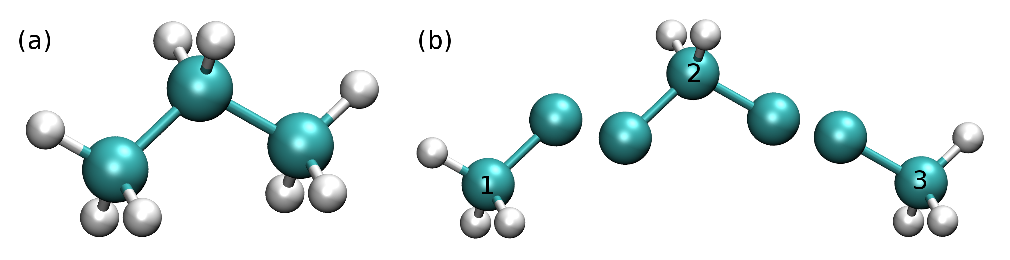
\includegraphics[width=0.99\textwidth]{c3}
	\caption{(a) An all-atom model of propane. (b) The same model as in (a), but parsed into three fragments.}
	\label{fig:propaneFragments}
\end{figure}


\begin{enumerate}
  \item Select the order in which each fragment of the ($N+1$)th molecule will be placed. The probability of the resulting sequence is $p_{seq}$. (See example in Table. \ref{table:propane}.)
  \begin{enumerate}
		\item The first fragment $i$ is chosen with uniform probability 1/$N_{frag}$.
    \item Subsequent fragments must be connected to a previously chosen fragment and are chosen with the uniform probability 1/$N_{cnxn}$, where the number of connections $N_{cnxn}= \sum_{ij}{\delta_{ij} h_{i} (1-h_{j})}$ is summed over all fragments $i$ and $j$. $h_i$ is 1 if fragment $i$ has been previously chosen and 0 otherwise. $\delta_{ij}$ is 1 if fragments $i$ and $j$ are connected and 0 otherwise.
  \end{enumerate}
	\item Select a conformation for fragment $i$ with Boltzmann probability \newline $e^{-\beta U(\mathbf{q}_{frag_i})}d\mathbf{q}_{frag_i}/Z_{frag_i}$, where $\mathbf{q}_{frag_i}$ are the internal degrees of freedom (angles and/or impropers) associated with fragment $i$.
	\item Select an orientation with uniform probability $d\mathbf{q}_{rot}/Z_{rot}$. 
	\item Select a coordinate for the center of mass (COM) of fragment $i$:
	\begin{enumerate}
		\item Select $\kappa_{ins}$ trial coordinates $\mathbf{r}_k$, each with uniform probability $d\mathbf{r}/V$. Since one of the trial coordinates will be selected later, the individual probabilities are additive. The probability of the collection of trial coordinates is $\kappa_{ins}d\mathbf{r}/V$.
		\item Compute the change in potential energy $\Delta U_k^{ins}$ of inserting fragment $i$ at each position $\mathbf{r}_k$ into configuration $\mathbf{q}_m^N$.
		\item Select one of the trial coordinates with probability $e^{-\beta \Delta U_k^{ins}} / \sum_k{e^{-\beta \Delta U_k^{ins}}}$.
	\end{enumerate}
	\item For each additional fragment $j$:
	\begin{enumerate}
		\item Select a fragment conformation with Boltzmann probability\newline$e^{-\beta U(\mathbf{q}_{frag_j})}d\mathbf{q}_{frag_j}/Z_{frag_j}$
		\item Select the first of $\kappa_{dih}$ trial dihedrals $\phi_0$ with uniform probability from the interval [0,$\frac{2\pi}{\kappa_{dih}}$). Additional trial dihedrals are equally spaced around the unit circle, $\phi_k=\phi_{k-1}+2\pi/\kappa_{dih}$. The probability of selecting $\phi_0$ is $\kappa_{dih}d\phi/2\pi$.
		\item Compute the change in potential energy $\Delta U_k^{dih}$ of attaching fragment $j$ to the growing molecule with each dihedral $\phi_k$.
		\item Select one of the trial dihedrals with probability $e^{-\beta \Delta U_k^{dih}} / \sum_k{e^{-\beta \Delta U_k^{dih}}}$.
	\end{enumerate}
\end{enumerate}

\begin{table}
\caption{Possible sequences and probabilities for inserting the fragments of the all-atom model of propane shown in Fig. \ref{fig:propaneFragments}.}
\label{table:propane}
\centering
\begin{tabular}{|c|c|} \hline
 {\bf Sequence} & {\bf $p_{seq}$} \\ \hline
 1 2 3 & 1/3 \\
 2 1 3 & 1/6 \\
 2 3 1 & 1/6 \\
 3 2 1 & 1/3 \\
 \hline
\multicolumn{2}{c}{}
\end{tabular}
\end{table}

The overall probability $\alpha_{mn}$ of attempting the insertion with the selected position, orientation and conformation is 

\begin{align}
\alpha_{mn} &= p_{seq}\ \frac{d\mathbf{q}_{rot}}{Z_{rot}}\ \frac{\kappa_{ins}d\mathbf{r}}{V}\ \frac{e^{-\beta \Delta U_k^{ins}}}{\sum_k{e^{-\beta \Delta U_k^{ins}}}}\ \times \nonumber \\
&\ \ \ \left[\prod_{i=1}^{N_{frag}}{\frac{e^{-\beta U(\mathbf{q}_{frag_i})}d\mathbf{q}_{frag_i}}{Z_{frag_i}}}\right]\ \left[\prod_{j=1}^{N_{frag}-1}{\frac{\kappa_{dih}d\phi}{2\pi}\ \frac{e^{-\beta \Delta U_k^{dih}}}{\sum_k{e^{-\beta \Delta U_k^{dih}}}}}\right] \\
\label{eq:alpha_cbmcInsert}
&= p_{seq}\ p_{bias}\ \frac{e^{-\beta U(\mathbf{q}_{frag})}d\mathbf{q}}{VZ_{rot}Z_{frag}\Omega_{dih}}
\end{align}

where $Z_{frag} = \prod_i Z_{frag_i}$ is the configurational partition function over degrees of freedom internal to each fragment, $U(\mathbf{q}_{frag}) = \sum_iU(\mathbf{q}_{frag_i})$ is the summed potential energy of each of the (disconnected) fragments, $\Omega_{dih} = (2\pi)^{N_{frag}-1}$ and $p_{bias}$ is

\begin{equation}
p_{bias} = \frac{\kappa_{ins}\ e^{-\beta \Delta U_k^{ins}}}{\sum_k{e^{-\beta \Delta U_k^{ins}}}}\ \left[\prod_{j=1}^{N_{frag}-1}{\frac{\kappa_{dih}\ e^{-\beta \Delta U_k^{dih}}}{\sum_k{e^{-\beta \Delta U_k^{dih}}}}}\right]
\end{equation}

Note that the term $VZ_{rot}Z_{frag}\Omega_{dih}$ in the denominator of Eq.\ (\ref{eq:alpha_cbmcInsert}) differs from $Z(1,V,T)=VZ_{rot}Z_{int}$.

In the reverse move, 1 of the $N+1$ particles is randomly selected for deletion. The probability $\alpha_{nm}$ of picking the molecule we just inserted is

\begin{equation}
\label{eq:alpha_cbmcReverseInsert}
\alpha_{nm} = \frac{1}{N+1}
\end{equation}

Combining Eqs.\ (\ref{eq:alpha_cbmcInsert}) and (\ref{eq:alpha_cbmcReverseInsert}) with Eq.\ (\ref{eq:pMuVT_ratio}) or Eq.\ (\ref{eq:pfVT_ratio}) gives the acceptance probability for a CBMC insertion move

\begin{align}
\label{eq:pAcc_cbmcInsertMuShift}
\ln\left( \frac{\alpha_{mn}}{\alpha_{nm}} \frac{p_m}{p_n} \right) &= \beta \left[\Delta U - U(\mathbf{q}^{(N+1)}_{frag,n})\right] - \beta \mu' + \ln\left( \frac{(N+1)\Lambda^3}{V} \right) + \ln\left( p_{seq}p_{bias} \right) \\
\label{eq:pAcc_cbmcInsertFShift}
&= \beta \left[\Delta U - U(\mathbf{q}^{(N+1)}_{frag,n})\right] + \ln\left( \frac{N+1}{\beta f' V} \right) + \ln\left( p_{seq}p_{bias} \right)
\end{align}

where $\mu'$ and $f'$ are, respectively, a shifted chemical potential and a skewed fugacity,

\begin{align}
\label{eq:muShift}
\mu'&=\mu+k_BT\ln\left( Q_{rot+int} \frac{Z_{frag}\Omega_{dih}}{Z_{int}} \right) \\
\label{eq:fShift}
f'&= f \frac{Z_{frag}\Omega_{dih}}{Z_{int}}
\end{align}

All of the terms in Eqs.\ (\ref{eq:muShift}) and (\ref{eq:fShift}) are intensive. GCMC simulations using Eqs.\ (\ref{eq:pAcc_cbmcInsertMuShift}) and (\ref{eq:pAcc_cbmcInsertFShift}) will converge to the same average density regardless of the simulation volume $V$. However, the values of $\mu'$ or $f'$ that correspond to the converged density will {\em not} match tabulated values of $\mu$ or $f$ computed from experimental data.

Note that the term $Z^{IG}/\Omega$ from Macedonia {\em et al}. would be equivalent to $Z_{int}/\Omega_{frag}\Omega_{dih}$ in the nomenclature used here. The configurational partition function of the disconnected fragments integrates over a Boltzmann factor, $Z_{frag} = \int e^{-\beta U(\mathbf{q}_{frag})} d\mathbf{q}_{frag}$, whereas the term $\Omega_{frag} = \int d\mathbf{q}_{frag}$ does not.

In Cassandra, the insertion move is implemented in the subroutine Insertion in insertion.f90. The relevant lines from version 1.1 are quoted below. The variable names in the insertion.f90 code are identified with symbols in Table \ref{table:cbmcInsert}.

\begin{minipage}{\linewidth}
\begin{lstlisting}[firstnumber=441, caption=insertion.f90]
  ln_pacc = beta(this_box) * (delta_e - E_angle - nrg_ring_frag_tot)
\end{lstlisting}
\begin{lstlisting}[firstnumber=447]
  ln_pacc = ln_pacc + DLOG(P_seq * P_bias) &
                    + DLOG(REAL(nmols(is,this_box)+1,DP)) &
                    - DLOG(box_list(this_box)%volume)

  IF(lchempot) THEN
     ! chemical potential is input
     ln_pacc = ln_pacc - species_list(is)%chem_potential * beta(this_box) &
               + 3.0_DP*DLOG(species_list(is)%de_broglie(this_box))
  ELSE   
     ! fugacity is input
     ln_pacc = ln_pacc - DLOG(species_list(is)%fugacity) &
                       - DLOG(beta(this_box)) &
  END IF 

  accept = accept_or_reject(ln_pacc)
\end{lstlisting}
\end{minipage}

\begin{table}
\caption{Variable symbols and code names for inserting a molecule}
\label{table:cbmcInsert}
\centering
\begin{tabular}{|c|c|} \hline
 {\bf Symbol} & {\bf Code name} \\ \hline
 $\beta$ & beta(this\_box) \\
 $\Delta U$ & delta\_e \\
 $U(\mathbf{q}_{frag})$ & E\_angle + nrg\_ring\_frag\_tot \\
 $p_{seq}$ & P\_seq \\
 $p_{bias}$ & P\_bias \\
 $\mu'$ & species\_list(is)\%chem\_potential \\
 $N$ & nmols(is,this\_box) \\
 $V$ & box\_list(this\_box)\%volume \\
 $\Lambda$ & species\_list(is)\%de\_broglie(this\_box) \\
 $f'$ & species\_list(is)\%fugacity \\
 \hline
\multicolumn{2}{c}{}
\end{tabular}
\end{table}

\subsection{Deleting a Molecule that was Inserted via \newline Configurational Bias Monte Carlo}
\label{sec:cbmcDelete}

The probability $\alpha_{mn}$ of choosing a molecule to delete is

\begin{equation}
\alpha_{mn} = \frac{1}{N}
\end{equation}

The probability of the reverse move $\alpha_{nm}$ requires knowledge of the sequence and biasing probabilities $p_{seq}$ and $p_{bias}$ that would have been used to place the molecule if it was being inserted. $p_{seq}$ and $p_{bias}$ can be calculated using the following procedure:

\begin{enumerate}
  \item Select the fragment order using the same procedure for inserting a molecule. The probability of the resulting sequence is $p_{seq}$.
	\item The first fragment in the sequence is fragment $j$. Calculate the intramolecular potential energy of fragment $j$'s current conformation, $U(\mathbf{q}_{frag_j})$. The probability of this conformation is Boltzmann  $e^{-\beta U(\mathbf{q}_{frag_j})}d\mathbf{q}_{frag_j}/Z_{frag_j}$.
	\item The probability of the fragment's current orientation is $d\mathbf{q}_{rot}/Z_{rot}$. 
	\item Calculate the weight of the fragment's current center of mass (COM) coordinates:
	\begin{enumerate}
		\item Compute the interaction potential energy $\Delta U^{ins}$ between fragment $j$ and the other $N-1$ molecules.
		\item Select $\kappa_{ins}-1$ trial coordinates $\mathbf{r}_k$, each with uniform probability $d\mathbf{r}/V$.
		\item Calculate the weight of the fragment's current COM amongst the trial coordinates, $e^{-\beta \Delta U^{ins}} / \sum_k{e^{-\beta \Delta U_k^{ins}}}$.
	\end{enumerate}
	\item For each additional fragment $j$:
	\begin{enumerate}
		\item Calculate the intramolecular potential energy of fragment $j$'s current conformation, $U(\mathbf{q}_{frag_j})$. The weight of this conformation in the Boltzmann distribution is $e^{-\beta U(\mathbf{q}_{frag_j})}d\mathbf{q}_{frag_j}/Z_{frag_j}$.
		\item Calculate the interaction potential energy $\Delta U^{dih}$ between fragment $j$, on the one hand, and fragments $i$ through $j-1$ and the other $N-1$ molecules.
		\item Calculate the current dihedral $\phi_0$ of fragment $j$. Compute the interaction potential energy $\Delta U_k^{dih}$ at $\kappa_{dih}-1$ trial dihedrals $\phi_k = \phi_{k-1} + 2\pi/\kappa_{dih}$.
		\item Compute the weight of $\phi_0$ amongst the trial dihedrals, $e^{-\beta \Delta U^{dih}}/ \sum_k{e^{-\beta \Delta U_k^{dih}}}$.
	\end{enumerate}
\end{enumerate}

The overall probability $\alpha_{nm}$ is 

\begin{equation}
\label{eq:alpha_cbmcReverseDelete}
\alpha_{nm} = p_{seq}\ p_{bias}\ \frac{e^{-\beta U(\mathbf{q}_{frag})}d\mathbf{q}}{VZ_{rot}Z_{frag}\Omega_{dih}}.
\end{equation}

The acceptance criteria for deleting a molecule inserted via CBMC is

\begin{align}
\label{eq:pAcc_cbmcDeleteMuShift}
\ln\left( \frac{\alpha_{mn}}{\alpha_{nm}} \frac{p_m}{p_n} \right) &= \beta \left[\Delta U + U(\mathbf{q}^{(i)}_{frag,m})\right] + \beta \mu' + \ln\left( \frac{V}{N\Lambda^3} \right) - \ln\left( p_{seq}p_{bias} \right) \\
\label{eq_pAcc_cbmcDeleteF}
&= \beta \left[\Delta U + U(\mathbf{q}^{(i)}_{frag,m})\right] + \ln\left( \frac{\beta f' V}{N} \right) - \ln\left( p_{seq}p_{bias} \right)
\end{align}

In Cassandra, the deletion move is implemented in the subroutine Deletion in deletion.f90. The relevant lines are quoted below. The variable names in deletion.f90 code are identified with symbols in Table \ref{table:cbmcDelete}.

\begin{minipage}{\linewidth}
\begin{lstlisting}[firstnumber=334, caption=deletion.f90]
  ln_pacc = beta(this_box) * (delta_e + E_angle + nrg_ring_frag_tot)
\end{lstlisting}
\begin{lstlisting}[firstnumber=340]
  ln_pacc = ln_pacc - DLOG(P_seq * P_bias) &
                    - DLOG(REAL(nmols(is,this_box),DP)) &
                    + DLOG(box_list(this_box)%volume)
 
  IF(lchempot) THEN
     ! chemical potential is input
     ln_pacc = ln_pacc + beta(this_box) * species_list(is)%chem_potential &
             - 3.0_DP*DLOG(species_list(is)%de_broglie(this_box))
  ELSE
     ! fugacity is input
     ln_pacc = ln_pacc + DLOG(species_list(is)%fugacity) &
                       + DLOG(beta(this_box)) &
  END IF
 
  accept = accept_or_reject(ln_pacc)

\end{lstlisting}
\end{minipage}

\begin{table}
\caption{Variable symbols and code names for deleting a molecule}
\label{table:cbmcDelete}
\centering
\begin{tabular}{|c|c|} \hline
 {\bf Symbol} & {\bf Code name} \\ \hline
 $\beta$ & beta(this\_box) \\
 $\Delta U$ & delta\_e \\
 $U(\mathbf{q}_{frag})$ & E\_angle + nrg\_ring\_frag\_tot \\
 $p_{seq}$ & P\_seq \\
 $p_{bias}$ & P\_bias \\
 $\mu'$ & species\_list(is)\%chem\_potential \\
 $N$ & nmols(is,this\_box) \\
 $V$ & box\_list(this\_box)\%volume \\
 $\Lambda$ & species\_list(is)\%de\_broglie(this\_box) \\
 $f'$ & species\_list(is)\%fugacity \\
 \hline
\multicolumn{2}{c}{}
\end{tabular}
\end{table}

\subsection{Regrowing a Molecule with Configurational Bias Monte Carlo}
\label{sec:cbmcRegrow}
Regrowing a molecule that has more than one fragment is a combination deletion and insertion move. Starting from microstate $m$:

\begin{enumerate}
	\item Randomly select a molecule with uniform probability $1/N$.
	\item Randomly select a bond to cut on the selected molecule with uniform probability $1/N_{bonds}$.
	\item Delete the fragments on one side of the bond or the other with equal probability. The number of deleted fragments is $N_{del}$.
	\item Reinsert the deleted fragments using the CBMC procedures for selecting the order of inserting the fragments, choosing a fragment conformation, and a connecting dihedral value (see Section \ref{sec:cbmcInsert}).
\end{enumerate}

The overall probability $\alpha_{mn}$ of attempting to regrow the molecule with the selected conformation is 

\begin{align}
\alpha_{mn} &= \frac{p_{seq}}{N N_{bonds}}\ \left[\prod_{j=1}^{N_{del}}{\frac{e^{-\beta U(\mathbf{q}^{(i)}_{frag_j})}d\mathbf{q}_{frag_j}}{Z_{frag_j}}}\right]\ \left[\prod_{j=1}^{N_{del}}{\frac{\kappa_{dih}d\phi}{2\pi}\ \frac{e^{-\beta \Delta U_k^{dih}}}{\sum_k{e^{-\beta \Delta U_k^{dih}}}}}\right] \nonumber \\
\label{eq:alpha_cbmcRegrow}
&= \frac{p_{seq}}{N N_{bonds}}\ \frac{e^{-\beta U(\mathbf{q}^{(i)}_{del,n})}d\mathbf{q}}{Z_{del}\Omega_{del}}\ p_{forward}
\end{align}

where $Z_{del} = \prod_i Z_{frag_j}$ is the configurational partition function over degrees of freedom internal to the deleted fragments, $U(\mathbf{q}^{(i)}_{del,n}) = \sum_jU(\mathbf{q}_{frag_j})$ is the summed potential energy of each deleted fragment with the conformations in microstate $n$, $\Omega_{del} = (2\pi)^{N_{del}}$ and $p_{forward}$ is the biasing probability

\begin{equation}
p_{forward} = \prod_{j=1}^{N_{del}}{\frac{\kappa_{dih}\ e^{-\beta \Delta U_k^{dih}}}{\sum_k{e^{-\beta \Delta U_k^{dih}}}}}
\end{equation}

The reverse move is identical except for the potential energy of the deleted fragments $U(\mathbf{q}^{(i)}_{del,m})$ in microstate $m$ and the biasing probability $p_{reverse}$ which will depend on the values of the connecting dihedrals. Using Eqs. (\ref{eq:pNVT_ratio}) and (\ref{eq:alpha_cbmcRegrow}), the acceptance criteria is:

\begin{equation}
\label{eq:pAcc_cbmcRegrow}
\ln\left( \frac{\alpha_{mn}}{\alpha_{nm}} \frac{p_m}{p_n} \right) = \beta \left[\left( U(\mathbf{q}^N_n) - U(\mathbf{q}^{(i)}_{del,n})\right) - \left(U(\mathbf{q}^N_m) - U(\mathbf{q}^{(i)}_{del,m})\right)\right] + \ln\left( \frac{p_{forward}}{p_{reverse}} \right)
\end{equation}

Eq. (\ref{eq:pAcc_cbmcRegrow}) is implemented in subroutine cut\_N\_grow() in file cutNgrow.f90. 

\begin{minipage}{\linewidth}
\begin{lstlisting}[firstnumber=392, caption=cutNgrow.f90, label=code:cbmcRegrow]
  ln_pacc = beta(this_box) * (delta_e_n - nrg_ring_frag_forward) &
          - beta(this_box) * (delta_e_o - nrg_ring_frag_reverse) &
          + DLOG(P_forward / P_reverse)

  accept = accept_or_reject(ln_pacc)
\end{lstlisting}
\end{minipage}

\begin{table}
\caption{Variable symbols and code names for regrowing a molecule}
\label{table:cbmcRegrow}
\centering
\begin{tabular}{|c|c|} \hline
 {\bf Symbol} & {\bf Code name} \\ \hline
 $\beta$ & beta(this\_box) \\
 $U(\mathbf{q}^N_n) - U(\mathbf{q}^{(i)}_{del,n})$ & delta\_e\_n - nrg\_ring\_frag\_forward \\
 $U(\mathbf{q}^N_m) - U(\mathbf{q}^{(i)}_{del,m})$ & delta\_e\_o - nrg\_ring\_frag\_reverse \\
 $p_{forward}$ & P\_forward \\
 $p_{reverse}$ & P\_reverse \\
 \hline
\multicolumn{2}{c}{}
\end{tabular}
\end{table}

\section{Multiphase Systems}
\label{sec:multiphase}
\subsection{Gibbs Ensemble Monte Carlo} 
\label{sec:gibbs}

[SECTION INCOMPLETE]

\section{Multicomponent Systems} 

Sections \ref{sec:NVT}-\ref{sec:multiphase} have each been developed for pure component systems. The Monte Carlo moves and acceptance criteria for multicomponent systems are straightforward extensions of the pure component moves. The only modification needed to translate, rotate and regrow molecules is to first select a species. In these moves, a species is selected randomly in proportion to its mole fraction $N_i/N$. When inserting and deleting a molecule, the mole fractions of each species change. In these cases, a species in a multicomponent system is selected instead with uniform probability $1/N_{species}$. In either case, species selection is symmetric for both forward and reverse moves and so cancels from the acceptance criterion.

In contrast, Reaction Ensemble Monte Carlo (RxMC) fundamentally occurs in a multicomponent grand canonical ensemble because the number of molecules of all species involved in a reaction change simultaneously. In the multicomponent grand canonical ensemble, the temperature $T$, volume $V$ and set of chemical potentials $\{\mu\} = \mu_1, \ldots, \mu_s$ of each species are held constant. The partition function for a system with $s$ species is

\begin{equation}
\label{eq:partitionFn_MuiVT}
\Xi(\{\mu\},V,T) = \sum\limits_{N_1=0}^{\infty} \ldots \sum\limits_{N_s=0}^{\infty}Q(\{N\},V,T)\ e^{\beta \mu_i N_i}
\end{equation}

where $\{N\}$ is the set of $s$ molecule numbers, and a summation is implied over the term $\mu_i N_i$. The probability of the system having $\{N\}$ molecules is 

\begin{equation}
\label{eq:pNi}
p(\{N\}) = \frac{Q(\{N\},V,T)e^{\beta \mu_i N_i}}{\Xi(\{\mu\},V,T)}
\end{equation}

The probability of observing microstate $m$ with $\{N\}_m$ molecules and configuration $\{\mathbf{q}^N\}_m$ is

\begin{align}
\label{eq:pMuiVT}
p_m &= \frac{e^{-\beta U_m} \prod\limits_{i=1}^s{d\mathbf{q}_i^{N_{im}}}}{Z(\{N\}_m,V,T)}\ \frac{Q(\{N\}_m,V,T)e^{\beta \mu_i N_{im}}}{\Xi(\{\mu\},V,T)} \nonumber \\
&= \frac{e^{-\beta U_m + \beta \mu_i N_{im}}}{\Xi(\{\mu\},V,T)}\ \prod\limits_{i=1}^s\left[\frac{Q_i(1,V,T)}{Z_i(1,V,T)}\ d\mathbf{q}_i\right]^{N_{im}}
\end{align}

The ratio of microstates is 

\begin{equation}
\label{eq:pMuiVT_ratio}
\frac{p_m}{p_n} = e^{\beta \Delta U - \beta \mu_i \Delta N_i}\ \prod\limits_{i=1}^s\left[\frac{Q_i(1,V,T)}{Z_i(1,V,T)}\ d\mathbf{q}_i\right]^{-\Delta N_i}
\end{equation}

\subsection{Reaction Ensemble Monte Carlo}
\label{sec:rxmc}
In Reaction Ensemble Monte Carlo, the number of molecules of each species can only change by a stoichiometric amount $\nu_i$ as a reaction occurs in the forward direction or $-\nu_i$ as a reaction occurs in the reverse direction. Moreover, reaction equilibrium occurs when the following condition is met

\begin{equation}
\label{eq:rxnEquil}
\sum\limits_{i=1}^{s}{\nu_i \mu_i} = 0
\end{equation}

Substituting Eq. (\ref{eq:rxnEquil}) and $\Delta N_i = \pm \nu_i$ into Eq. (\ref{eq:pMuiVT_ratio}) gives

\begin{equation}
\label{eq:pMuiVT_ratio_2}
\frac{p_m}{p_n} = e^{\beta \Delta U}\ \prod\limits_{i=1}^s\left[\frac{Q_i(1,V,T)}{Z_i(1,V,T)}\ d\mathbf{q}_i\right]^{\mp \nu_i}
\end{equation}

The product of partition functions can be replaced by the equilibrium constant of an ideal gas $K_{eq}$ or the standard change of free energy $\Delta G_{rxn}^o$

\begin{equation}
\label{eq:Keq_ideal}
\prod\limits_{i=1}^s{\left(\frac{Q_i(1,V,T)}{V}\right)^{\nu_i}} = K_{eq} = e^{-\beta \Delta G_{rxn}^o} (P\degree k_BT)^{\Delta \nu}
\end{equation}

where $P\degree$ is the standard pressure (by default, 1 atm). Substituting Eq. (\ref{eq:Keq_ideal}) and $Z(1,V,T) = VZ_{rot}Z_{int}$ into Eq. (\ref{eq:pMuiVT_ratio_2}) gives

\begin{align}
\label{eq:pMuiVT_ratio_3}
\frac{p_m}{p_n} &= e^{\beta \Delta U}\ K_{eq}^{\mp 1}\ \prod\limits_{i=1}^s\left[\frac{d\mathbf{q}_i}{Z_{rot,i}Z_{int,i}}\right]^{\mp \nu_i} \\
&= e^{\beta \Delta U \pm \beta \Delta G_{rxn}^o}\ \prod\limits_{i=1}^s\left[\frac{d\mathbf{q}_i}{P\degree k_BT\ Z_{rot,i}Z_{int,i}}\right]^{\mp \nu_i}
\end{align}

\section{Appendix}
\label{sec:appendix}
\subsection{Inserting a Molecule Randomly}
\label{sec:randomInsert}
To insert a molecule, a position, orientation and molecular conformation must each be selected. The probability of inserting the new molecule at a random location is $d\mathbf{r}/V$, where $d\mathbf{r}$ is a Cartesian volume element of a single atom. The probability of choosing the molecule orientation is $d\mathbf{q}_{rot}/Z_{rot}$, which for a linear molecule is $d \cos(\theta) d\phi / 4\pi$ and for a nonlinear molecule is $d \cos(\theta)d\phi d\psi/8\pi^2$. The probability of the molecule conformation only depends on the remaining $2M-5$ internal bond angles, dihedral angles and improper angles $\mathbf{q}_{int}$. A thermal ensemble of configurations is Boltzmann distributed $e^{-\beta U(\mathbf{q}_{int})}/Z_{int}$. The overall probability $\alpha_{mn}$ is

\begin{equation}
\alpha_{mn} = \frac{d\mathbf{r}}{V}\ \frac{d\mathbf{q}_{rot}}{Z_{rot}}\ \frac{e^{-\beta U(\mathbf{q}_{int,N+1,n})}}{Z_{int}}\ d\mathbf{q}_{int} = \frac{e^{-\beta U(\mathbf{q_{N+1,n}})}}{Z(1,V,T)}\ d\mathbf{q}.
\end{equation}

where we have used Eq.\ (\ref{eq:configPartitionFn_1VT}) to recover $Z(1,V,T)$ and recognized that only internal degrees of freedom contribute to the potential energy of the isolated $N+1$th molecule in microstate $n$, $U(\mathbf{q}_{N+1,n}) = U(\mathbf{q}_{int,N+1,n})$. For a point particle with no rotational or internal degrees of freedom, $\alpha_{mn}$ reduces to $d\mathbf{r}/V$. For molecules with internal flexibility, a library of configurations distributed according to $e^{-\beta U(\mathbf{q}_{int})}/Z_{int}$ can be generated from a single molecule MC simulation. In the reverse move, 1 of the $N+1$ particles is randomly selected for deletion. The probability $\alpha_{nm}$ of picking the molecule we just inserted is

\begin{equation}
\alpha_{nm} = \frac{1}{N+1}
\end{equation}

The acceptance probability for a random insertion move is 

\begin{equation}
\label{eq:pAcc_randomInsertMu}
\ln\left( \frac{\alpha_{mn}}{\alpha_{nm}} \frac{p_m}{p_n} \right) = \beta \left[\Delta U - U(\mathbf{q}_{N+1})\right] - \beta \mu + \ln\left( \frac{N+1}{Q(1,V,T)} \right)
\end{equation}

where $U(\mathbf{q}_{N+1})$ is the intramolecular potential energy of the inserted molecule. $Q(1,V,T)$ is typically not known {\em a priori}, nor is it easily estimated. Substituting Eq.\ (\ref{eq:partitionFn_1VT}) into Eq.\ (\ref{eq:pAcc_randomInsertMu}) and absorbing $Q_{rot+int}$ into a shifted chemical potential $\mu'$

\begin{equation}
\mu' = \mu - k_BT\ln(Q_{rot+int})
\end{equation}

gives the acceptance criteria for inserting a molecule

\begin{equation}
\label{eq:pAcc_randomInsertMuShift}
\ln\left( \frac{\alpha_{mn}}{\alpha_{nm}} \frac{p_m}{p_n} \right) = \beta \left[\Delta U - U(\mathbf{q}_{N+1})\right] - \beta \mu' + \ln\left( \frac{(N+1)\Lambda^3}{V} \right).
\end{equation}

The terms absorbed into $\mu'$ are intensive and therefore GCMC simulations using Eq.\ (\ref{eq:pAcc_randomInsertMuShift}) will converge to a specific average density. However, the value of $\mu'$ that corresponds to the converged density will {\em not} match tabulated values of $\mu$ computed from experimental data.

Substituting Eq.\ (\ref{eq:mu}) into Eq.\ (\ref{eq:pAcc_randomInsertMu}) gives

\begin{equation}
\label{eq:pAcc_randomInsertF}
\ln\left( \frac{\alpha_{mn}}{\alpha_{nm}} \frac{p_m}{p_n} \right) = \beta \left[\Delta U - U(\mathbf{q}_{N+1})\right] + \ln\left( \frac{N+1}{\beta f V} \right)
\end{equation}

where no terms have been absorbed into the fugacity $f$. Note also that the partition function has completely been eliminated from the acceptance criteria.

\subsection{Deleting a Molecule Inserted Randomly}
\label{sec:randomDelete}

The probability $\alpha_{mn}$ of choosing a molecule to delete is

\begin{equation}
\alpha_{mn} = \frac{1}{N}
\end{equation}

The probability $\alpha_{nm}$ of inserting that molecule back in is

\begin{equation}
\alpha_{nm} = \frac{e^{-\beta U(\mathbf{q})}}{Z(1,V,T)}\ d\mathbf{q}
\end{equation}

The acceptance probability for deleting a molecule inserted randomly is

\begin{align}
\label{eq:pAcc_randomDeleteMuShift}
\ln\left( \frac{\alpha_{mn}}{\alpha_{nm}} \frac{p_m}{p_n} \right) &= \beta \left[\Delta U + U(\mathbf{q}_{N})\right] + \beta \mu' + \ln\left( \frac{V}{N\Lambda^3} \right) \\
\label{eq:pAcc_randomDeleteF}
&= \beta \left[\Delta U + U(\mathbf{q}_{N})\right] + \ln\left( \frac{\beta f V}{N} \right)
\end{align}

Note that in $\Delta U$ is defined differently in Eqs.\ (\ref{eq:pAcc_randomInsertMuShift}) and (\ref{eq:pAcc_randomInsertF}) than in Eqs.\ (\ref{eq:pAcc_randomDeleteMuShift}) and (\ref{eq:pAcc_randomDeleteF}). In the former, the new configuration has more molecules, $\Delta U = U(\mathbf{q}_n^{N+1}) - U(\mathbf{q}_m^N)$. In the latter, the new configuration has fewer molecules, $\Delta U = U(\mathbf{q}_n^{N-1}) - U(\mathbf{q}_m^N)$.
